\newcommand{\scaler}{0.6}
\newcommand{\plytawidth}{10cm*\scaler}
\newcommand{\plytalength}{2.5cm*\scaler}
\newcommand{\plytaheight}{5cm*\scaler}
\newcommand{\railcoor}{2cm*\scaler}
\newcommand{\railwidth}{0.4cm*\scaler}
\newcommand{\railheight}{0.6cm*\scaler}
\newcommand{\xots}{0.5cm*\scaler}
\newcommand{\eots}{0.15cm*\scaler}
\newcommand{\diagox}{0.1cm*\scaler}
\newcommand{\pressx}{1cm*\scaler}
\newcommand{\pressy}{0.5cm*\scaler}
\newcommand{\diagx}{0.15cm*\scaler}
\newcommand{\diagy}{0.15cm*\scaler}
\newcommand{\stalplytax}{0.2cm*\scaler}
\newcommand{\stalplytay}{1.5cm*\scaler}
\newcommand{\arrowlength}{0.6cm*\scaler}
\newcommand{\newgeom}{5cm*\scaler}
\newcommand{\newgeomx}{8cm*\scaler}
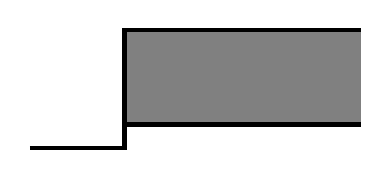
\begin{tikzpicture}
  \coordinate (A1) at (0, \pressy);
  \coordinate (B1) at (0, \plytalength);
  \coordinate (C1) at (\plytawidth/2, \pressy);
  \coordinate (D1) at (\plytawidth/2, \plytalength);
  \coordinate (E1) at (-\railcoor, 0);
  \coordinate (F1) at (-\railcoor, \plytalength);
  \coordinate (H1) at (0,  0);
  \coordinate (G1) at (\plytawidth, 0);
   
  \draw [ultra thick, fill=gray] (C1) -- (A1) -- (B1) -- (D1);
  \draw [ultra thick] (E1) -- (H1) -- (A1);
  
\end{tikzpicture}